%--------------------------------------------------------------------------------
%
% Text p��sp�vku do sborn�ku EEICT
%
% Vytvo�il:  Martin Drahansk�
% Datum:     26.02.2007
% E-mail:    drahan@fit.vutbr.cz
%
%--------------------------------------------------------------------------------
%
% P�elo�en�: pdflatex prispevek.tex
%
% Optim�ln� zp�sob pou�it� = p�epi�te jen vlastn� text
%
\documentclass{eeict}
\inputencoding{cp1250}
\usepackage[bf]{caption}
\usepackage{url}

%--------------------------------------------------------------------------------

\title{Design and Performance Analysis of Parallel Processing of SRTP Packets}
\author{Jan Wozniak}
\programme{Master Degree Programme (2), FIT BUT}
\emails{xwozni00@stud.fit.vutbr.cz}

\supervisor{Peter Jurne�ka}
\emailv{ijurnecka@fit.vutbr.cz}

\abstract{Encryption of real-time multimedia data transfers is one
  of the tasks for telecommunication infrastructure which should be considered
  in order to reach essential level of security. Execution time of ciphering 
  algorithm could play fundamental role in delay of the packets, therefore, it 
  provides interesting challenge in terms of optimization methods. This work 
  focuses on parallelization possibilities of processing SRTP for the 
  purposes of private gateway with the usage of OpenCL framework, utilization
  gateway's resources and analysis of potential improvement.}
\keywords{AES, SRTP, general-purpose GPU, OpenCL, parallel computations, 
  gateway, VoIP.}

\begin{document}
% -- Hlavi�ka pr�ce --

\maketitle

%-------------------------------------------------------------------------------
\selectlanguage{english}
\section{Introduction}
One of the essential metrics for measuring VoIP gateway's performance is 
the number and quality of simultaneous calls. It is affected mostly by the
computational demands of used communication protocols and number of registered
users. While the count of registered users provides very limited room for 
improvement by the nature of the problem itself, there could be wide variety
of approaches in implementing the protocol stacks. 

Significant amount of resources are utilized during indirect simultaneous call
sessions by processing multimedia packets \cite{analysis}. Since security has recently grown 
to be necessary feature in VoIP communication, and the encryption and decryption
processes are designed with the idea of optimization, it is primary scope of 
interest of this paper.

%Development and results in the areas of parallel architectures shows that many
%procedures could be distinctively accelerated by executing the algorithm on the
%processing unit capable of parallel computations. Therefore, this paper aims on
%implementation and analysis of parallel processing of encrypted real-time 
%multimedia data transferes.

\section{SRTP Processing}
Secure Real-time Transport Protocol was designed as an extension over RTP protocol
to obtain security and confidentiality for multimedia sessions on application layer
of ISO/OSI model. 

In VoIP communication the time has essential impact on the quality of
transmitted information, therefore, it is important that ensuring the 
security of RTP wouldn't increase the latency over the acceptable level.
Among typical limitations of real-time communications 
belong \cite{perkins:rtp2003}:
\vspace{-0.5em}
\begin{itemize}
\vspace{-0.5em}
\item Maximal tolerable latency of round-trip time 300~ms.
\vspace{-0.5em}
\item Smaller packet loss than 5\%.
\vspace{-0.5em}
\item Sensitivity to factors that are difficult to objectively measure
such as jitter.
\end{itemize}
\vspace{-1em}

The designed application captures data from network in the \textit{network layer} which 
ensures communication with both endpoints of multimedia session and is running in its own 
thread. It contains buffer pools for incoming and outgoing data to ensure maximal level 
of parallelization in each layer of application. Pointers for input and output buffers are 
passed for further packet processing where are extracted information such as header and payload 
from the packet, copied data from the memory to OpenCL data structures and serial implementation 
of AES key schedule. Parallel processing of payload is executed in precisely 16 work-items
while the application follows paradigm of persistent thread implementation. 

In the scheme in figure \ref{scheme} gray blocks visualize serial implementation in C/C++ and
yellow blocks are parallel implementation in OpenCL. The arrows represent data flows between
and inside of blocks. Thin purple lines depict usage of barriers.

Scheme \ref{scheme} visualizes only packet encoding, however, decoding is executed in similar manner.
The exact size of payload in SRTP packet can differ widely according to the 
used codec, its bit rate, and sampling frequency. The basic multimedia codec 
is G.711, which should be supported by every multimedia device and with standardly 
used 20ms sampling period, the length of payload is 160 bytes. Due to it's wide
support it has been chosen and used for evaluation and comparison of two approaches 
for encryption and decryption -- serial and parallel.

\begin{figure}[h!]
\centering
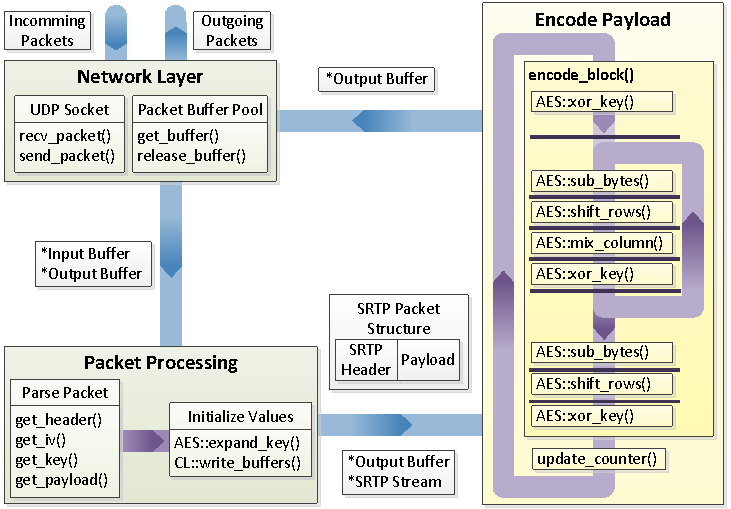
\includegraphics[width=15cm]{paral_scheme.pdf}
\caption{SRTP Parallel Processing Scheme.}
\label{scheme}
\end{figure}

\vspace{-1em}

\subsection{AES}
The CTR has been selected for the VoIP sessions due to its invariace
for delay and even possible loss of packets and it provides flexibility in SRTP processing
for packets received out of order. 
Each byte in the block of AES cipher can be computed separately. The local dependency
of bytes is limited to the distinct steps of the algorithm which requires usage of
barriers for local synchronization.

\subsection{Persistent Thread}
For massive parallel applications the obvious approach would be to utilize as much
of machine's power as possible to gain the largest speed-up in every single
execution. However, the aim of this paper is to minimize large delays for multiple 
sessions which requires rather careful allocation of resources. Persistent threads
is special type of programing paradigm combining both, the possible gain of mapping
the program for parallel computation and considerate usage of resources \cite{pt}.

Since the initialization of computational kernel can consume significant amount of
time compared to the actual execution, larger kernel reusing its resources
for multiple similar computations could render the initialization negligible trading
off portion of parallelization.
This approach has been chosen for packet parsing, while instead of mapping 160 OpenCL
work-items on the G.711 packet's payload it uses 16 work-items in a loop that 
goes through the data.

\section{Results}
The commercial gateway with optimized hardware can hold around 120 concurrent
calls \cite{hp4k}.
The evaluation of implementation proposed as backup for this paper is summarized
in following graphs of distributed packet latencies. Measured was round-trip time latency
of each packet during 50 to 150 concurrent calls that all lasted 20 seconds,  
results for 150 concurrent calls for serial implementation were excessively 
large thus not included in the graph. The thicker part of the column guarantees 
to contain 95\% of the packets which was earlier presented as one of requirements
for reliable session. 

The tests were all done on the machine with processor intel i5 2500k with HD3000 graphics chip
running OpenSUSE 12.2 and OpenCL version 1.2.


\begin{figure}[h!]
\centering
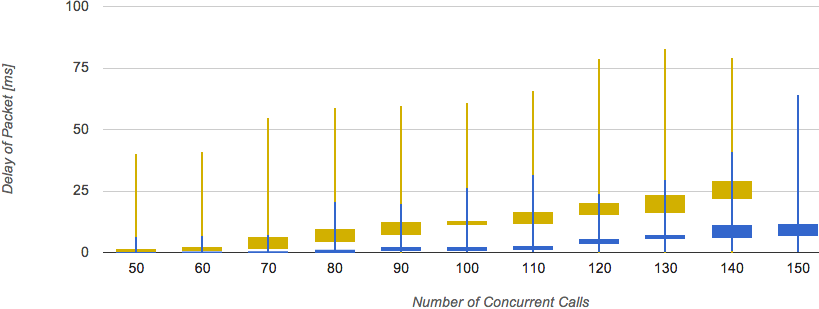
\includegraphics[width=14.7cm]{compare.png}
\vspace{-0.5em}
\caption{Latencies for parallel implementation in blue color and serial in yellow color.}
\end{figure}

\vspace{-1.1em}

\section{Conclusion}
Proposed parallel implementation can reduce packet latency caused by encryption 
to half or third depending on number of concurrent calls. Even though 
optimizations are far from being complete the results are promising and can bring
opportunities for improvement in related tasks, e.g. transcoding.

\vspace{-0.2em}
%\footnote{\url{http://www.athlsolutions.com/web/en/Products/tabid/128/ProdID/38/Hipath\_4000.aspx}}. 
%------------
% Citace
%
%\begin{thebibliography}{9}
%  \bibitem{rybicka} Rybi�ka, J.: \LaTeX pro za��te�n�ky, Brno, Konvoj 1999,
%            ISBN 80-85615-77-0
%  \bibitem{orsag} Ors�g, F.: Vision f�r die Zukunft. Biometrie, Kreutztal,
%            DE, b-Quadrat, 2004, s. 131-145, ISBN 3-933609-02-X
%  \bibitem{drahansky} Drahansk�, M., Ors�g, F.: Biometric Security Systems:
%    Robustness of the Finger-print and Speech Technologies. In: BT 2004 - 
%    International Workshop on Biometric Technologies, Calgary, CA, 2004,
%    s. 99-103
%\end{thebibliography}

\bibliography{literatura} % viz. literatura.bib
\bibliographystyle{ieeetr}
\end{document}
